%==============================================================================
\chapter{Fundamentos}\label{fundamentos}
%==============================================================================

Devido aos impasses demonstrados no \autoref{oproblema}, este trabalho é baseado em conceitos de aprendizado de máquina, que dedica-se na elaboraçãode algoritmos e técnicas que permitem um computador a aprender padrões.  

\section{Aprendizado de máquina}\label{sec:aprendizadodemaquina}

Para realizar a aprendizagem é necessário primeiramente dados de entrada que servem como exemplo para nosso modelo, com esses dados é possível treinar o modelo para que ele possa então aprender com base nesses exemplos. Depois de realizar o treinamento, é possível generalizar sobre outros dados ainda não testados e gerar uma resposta apropriada como saída. O diagrama da \autoref{fig:passoapasso} abaixo mostra os passos para obter o resultado final.

\begin{figure}[htb]
	  \caption{Diagrama para resultado final}\label{fig:passoapasso}
	  \begin{center}
	      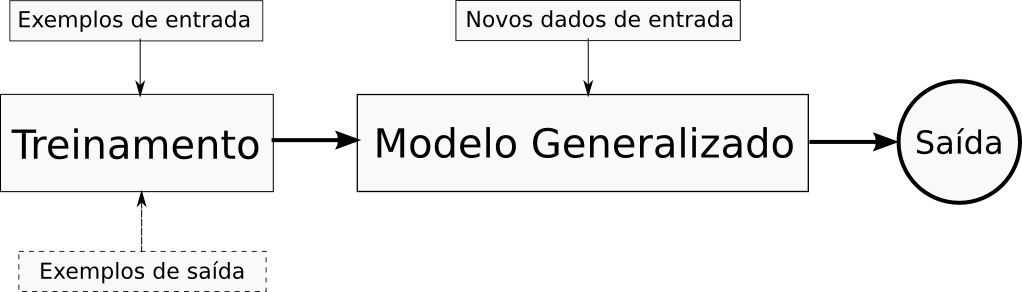
\includegraphics[scale=0.5]{img/passoapasso}
	  \end{center}
\end{figure}


O aprendizado de máquina pode ser dividido em duas abordagens: O \textbf{aprendizado supervisionado}, onde é dado um conjunto de dados de entrada e já se sabe como a saída deve parecer, tendo a ideia de que há uma relação entre a entrada e a saída; O \textbf{aprendizado não supervisionado}, que nos permite abordar problemas com pouca ou até nenhuma ideia de como os resultados devem parecer, nesse caso a caixa de exemplos de saída pode não existir.

Neste trabalho a abordagem utilizada vai ser o aprendizado supervisionado, pois já temos uma classe gramatical apropriada para cada palavra em seu contexto.

O aprendizado supervisionado permite dividir os problemas em duas categorias distintas:


\begin{itemize}
	\item \textbf{Regressão}: Tenta-se prever resultados com uma saída contínua, significando que deseja-se mapear variáveis de entrada em alguma função contínua. A \autoref{fig:demregressao} demonstra esse processo. Nessa demonstração, os círculos em vermelho são dados de exemplo, já a reta azul representa a predição feita pela regressão.
	\item \textbf{Classificação}:  Tenta-se prever resultados em uma saída discreta, ou seja, deseja0se mapear variáveis de entrada em categoriais discretas. A \autoref{fig:demclassificacao} demonstra esse processo. Essa demonstração tem duas classes diferentes, as representadas pelos círculos amarelos e pelas cruzes vermelhas, já o contorno em verde representa o resultado da classificação sobre esses dados de exemplo.
\end{itemize}


\begin{figure}[htb]
	  \caption{Demonstração de regressão}\label{fig:demregressao}
	  \begin{center}
	      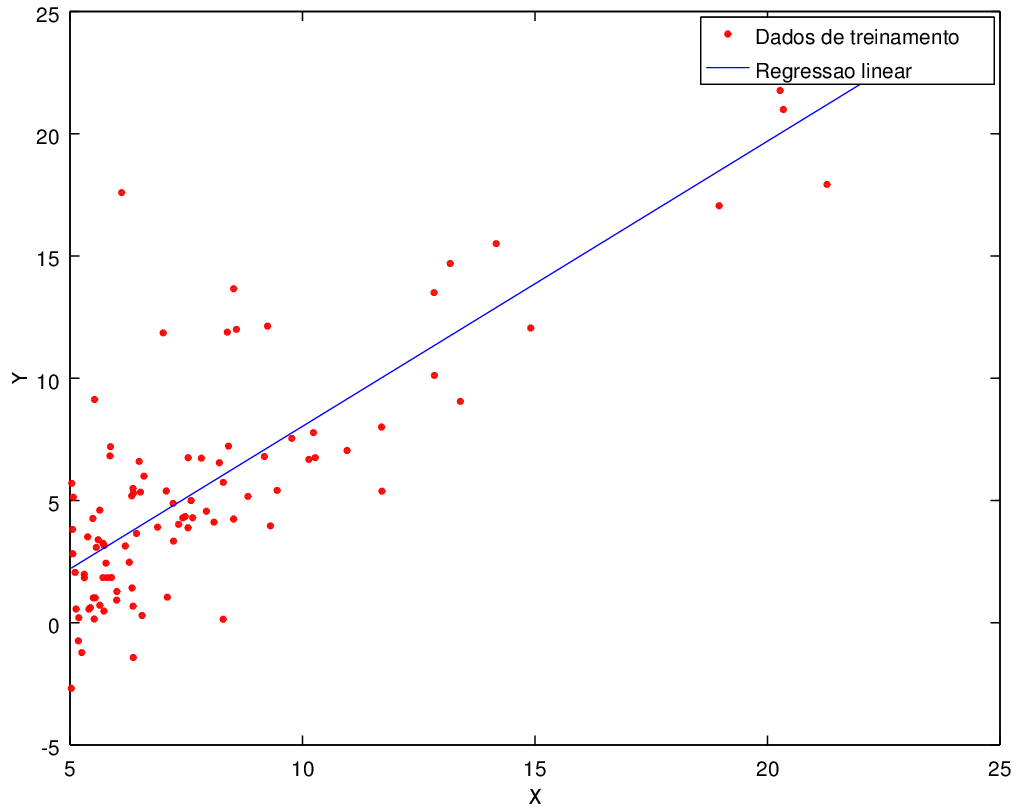
\includegraphics[scale=0.75]{img/regressao2}
	  \end{center}
	  \legend{Fonte: \cite{machinelearningcoursera}.}
\end{figure}

\begin{figure}[htb]
  \caption{Demonstração de classificação}\label{fig:demclassificacao}
  \begin{center}
      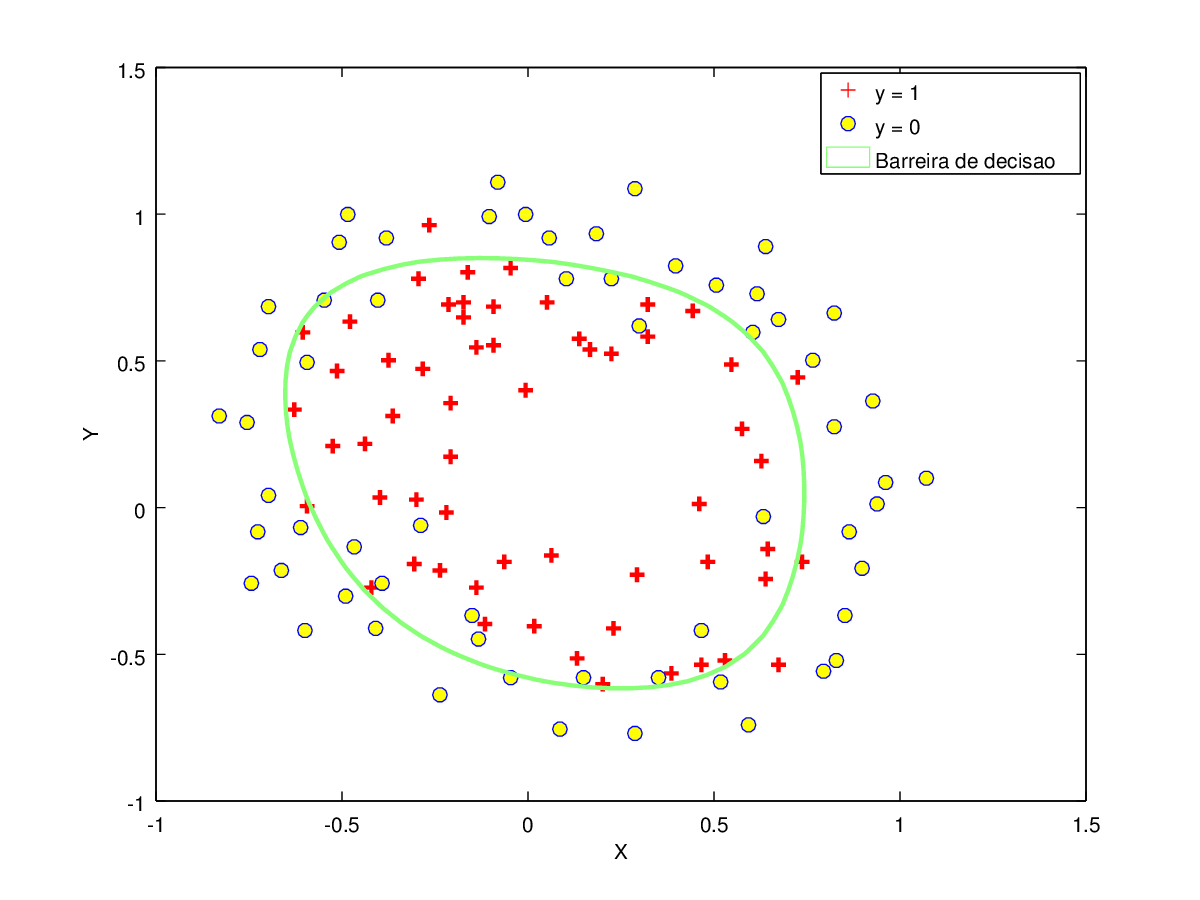
\includegraphics[scale=0.75]{img/classificacao2}
  \end{center}
  \legend{Fonte: \cite{machinelearningcoursera}.}
\end{figure}


Logo adiante será explicado os fundamentos de classificação e uma técnica para resolver esse problema chamada de regressão logística \cite{hosmer2004applied}. E em virtude de apresentar conceitos fundamentais há serem aplicados posteriormente nas redes neurais profundas, será falado um pouco mais sobre regressão logística, e também sobre propriedades importantes que serão referenciadas durante todo o trabalho.

\subsection{Classificação}

Em um problema de classificação, nossa saída \textit{Y} vai ser um vetor com valores sendo apenas zero ou um.

\begin{equation}\label{eq:binaryclassification}
Y \in \{0, 1\}
\end{equation}

A equação \ref{eq:binaryclassification} está tratando apenas duas classes. Sendo assim, esse problema é chamado de classificação binária. Para resolver esse problema, um método que pode ser utilizado é regressão logística.

A fim de simplificar o uso das variáveis, faremos o uso de uma notação que é normalmente utilizada em textos de aprendizado de máquina, ela pode ser vista na \autoref{tab:classificacaonomenclatura}.

\begin{table}[!htb]
\caption{Nomenclaturas} \label{tab:classificacaonomenclatura}
\begin{center}
\begin{tabular}{m{2cm}m{14.0cm}}
  \toprule
  $X$ & dados de entrada ou \textit{features} \\
  $Y$ & dados de saída \\
  $X_j^{(i)}$ & o valor da \textit{feature} \textit{j} no i-ésimo exemplo de treinamento \\
  $X^{(i)}$ & o vetor coluna de todas as \textit{features} no i-ésimo exemplo de treinamento \\
  $m$ & número de exemplos de treinamento \\
  $n$ & $|X^{(i)}|$, o número de \textit{features} \\
  $(x, y)$ & um exemplo de treinamento \\
  $(X^{(i)}, Y^{(i)})$ & o i-ésimo exemplo de treinamento \\
  $\theta$ & parâmetros a serem aprendidos \\
  \bottomrule
\end{tabular}
\legend{Notação utilizada para classificação}
\end{center}

\end{table}



\ \\
\ \\

\subsection{Função de hipótese}

A função de hipótese descreve a confiança dos dados de entrada para os dados de saída, para isso é atribuido valores para os parâmetros $\theta$s. Essa relação está definida na \autoref{eq:funcaodehipotese}. Observe que ela tem apenas dois parâmetros. Na realidade uma hipótese pode ter vários parâmetros relacionados com os dados de entrada \textit{X}, se tiver \textit{n} dados de entrada, então haverá \textit{n+1} parâmetros. A forma geral da função de hipótese está mostrada na \autoref{eq:funcaodehipotesegeral}.

\begin{align}
h_{\theta}(x) = &\ \theta_0 + \theta_1 x \label{eq:funcaodehipotese} \\
h_{\theta}(x) = &\ \theta_0 + \theta_1 x_1 + \theta_2 x_2 + ... + \theta_n x_n \label{eq:funcaodehipotesegeral}
\end{align}

Uma maneira de simplificar a função de hipótese é trabalhar com a definição de multiplicação de matrizes. Então a função de hipótese pode ser representada de uma forma vetorizada, como mostrado na \autoref{eq:funcaodehipotesegeralvet}.

\begin{equation}
h_{\theta}(x) = \big[\theta_0\ \theta_1\ ...\ \theta_n\big] \times \begin{bmatrix} x_0 \\ x_1 \\ \vdots \\ x_n \end{bmatrix}  = \theta^TX \label{eq:funcaodehipotesegeralvet}
\end{equation}

Para que seja possível fazer operações de matrizes com $\theta$ e $X$, será setado $X_0^{(i)} = 1$ para todos os valores de $i$. Isso faz com que os vetores $\theta$ e $X^{(i)}$ combinem um com o outro elementarmente.

Uma função de hipótese tem o objetivo de mapear funções aleatórias dentro do intervalo de saída \textit{Y}. Portanto, nossa função de hipótese deve satisfazer a \autoref{eq:reglogicfuncaohip}.

\begin{equation}\label{eq:reglogicfuncaohip}
0 \leq h_{\theta}(x) \leq 1
\end{equation}

Para fazer com que uma entrada contínua fique nesse intervalo, é necessário utilizar uma função linear que faça esse mapeamento de modo linear, e para isso mudamos a forma da função de hipótese. A nova forma usa a função sigmoide, também conhecida como função logística.

\begin{align}
h_{\theta}(x) = g(\theta^TX) \nonumber \\
z = \theta^TX \nonumber \\
g(z) = \frac{1}{1 + e^{-z}} \label{eq:funcaosigmoide}
\end{align}

\begin{figure}[htb]
  \caption{Função sigmoide}\label{fig:funcaosigmoide}
  \begin{center}
      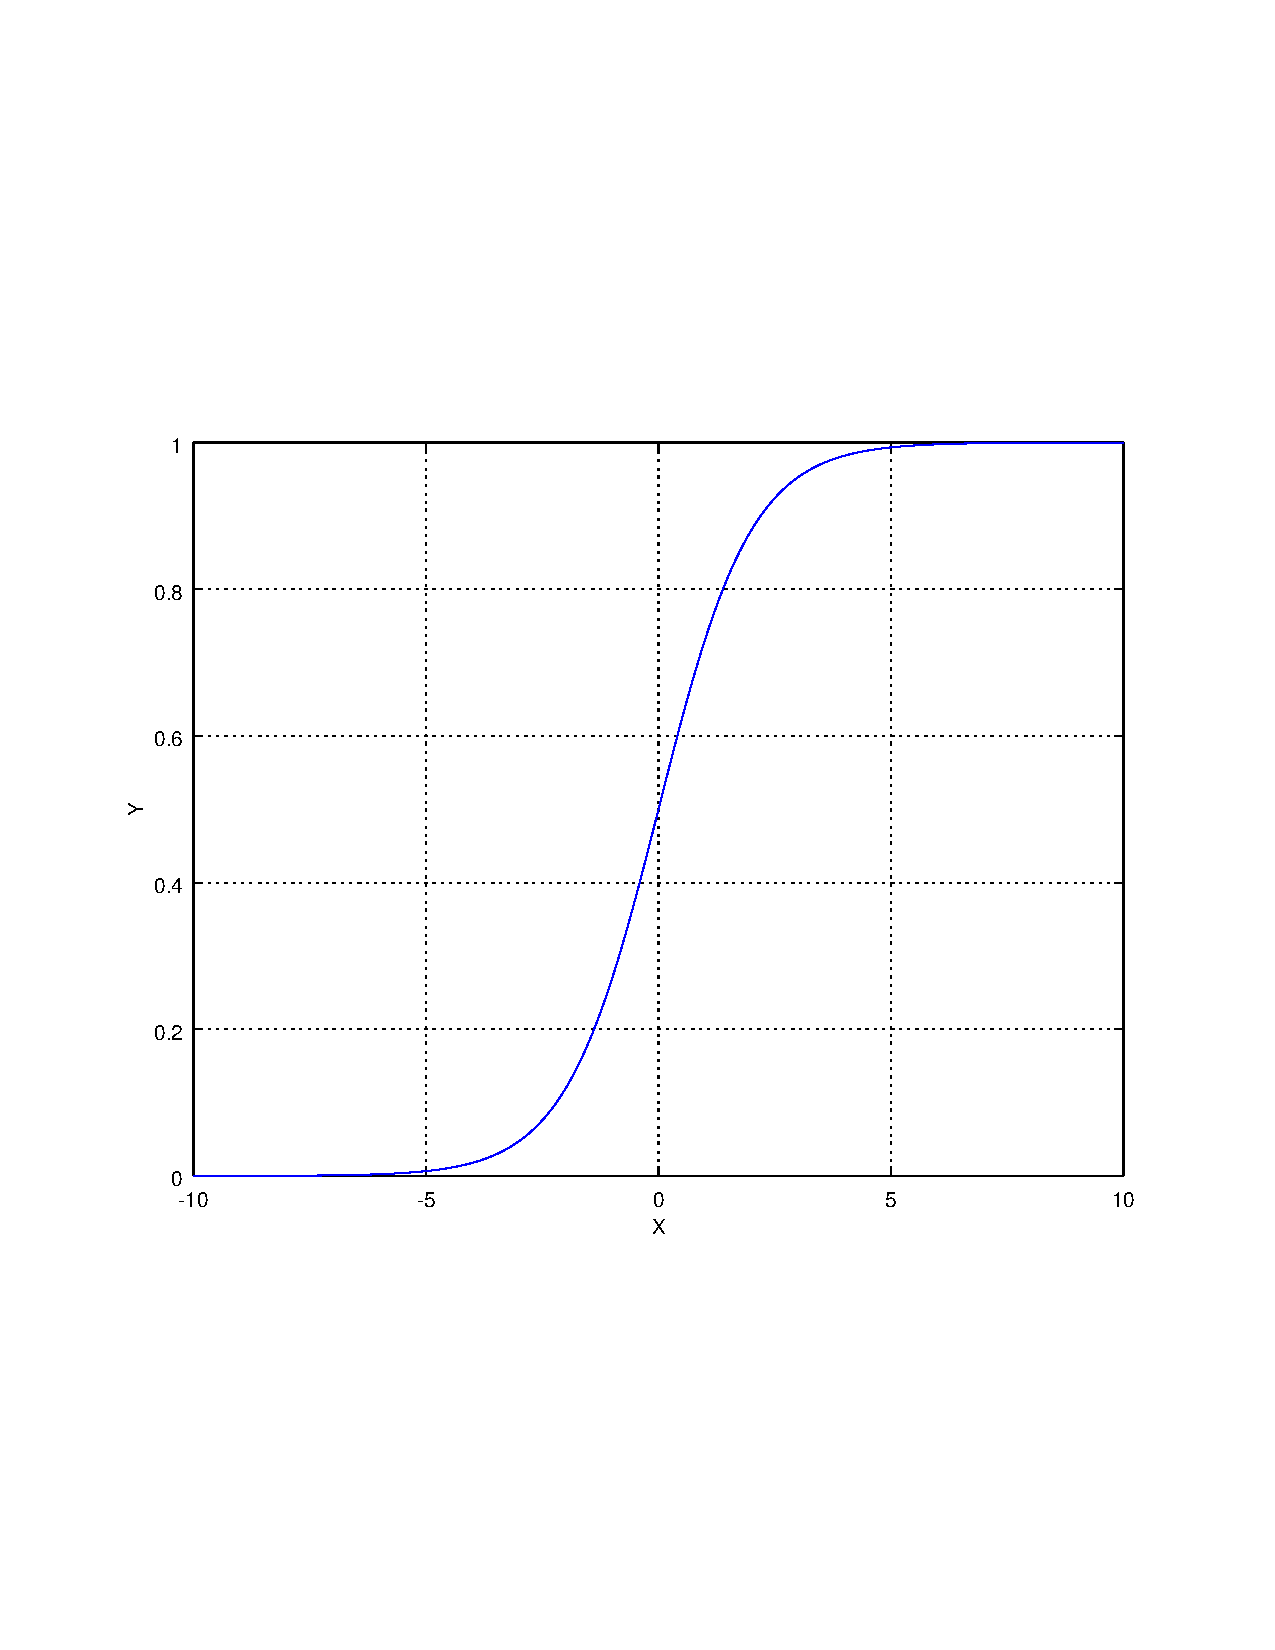
\includegraphics[scale=0.75]{img/funcaosigmoide}
  \end{center}
\end{figure}

A função da \autoref{eq:funcaosigmoide} representada na fígura \autoref{fig:funcaosigmoide} mapeia qualquer número no intervalo [0, 1], tornando isso útil para transformar qualquer valor arbitrário em uma função mais ideal para problemas de classificação.

Para calcular a função de hipótese, podemos colocar o $\theta^TX$ na função logística. Isso nos dará a probabilidade de que a saída é 1.

\begin{equation}
h_{\theta}(x) = P(y=1 | X ; \theta) = 1 - P(y=0 | X ; \theta) \nonumber
\end{equation}

Ou seja, a probabilidade de nossa predição ser 1 é o oposto da probabilidade de ser 0. Sendo assim, a soma das probabilidades para \textit{y = 0} e \textit{y = 1} deve ser 1.

Para de ter a classificação discreta podemos traduzir a saída da função de hipótese de acordo com a \autoref{eq:decisionboundary}:
\begin{align} 
h_{\theta}(x) \geq 0.5 \Rightarrow y = 1 \nonumber \\
h_{\theta}(x) < 0.5 \Rightarrow y = 0 \label{eq:decisionboundary}
\end{align}

Então, se a entrada é $\theta^TX$, isso significa que:
\begin{equation}
h_{\theta}(x) = g(\theta^TX) \geq 0.5 \quad \text{ quando } \quad \theta^TX \geq 0 \nonumber
\end{equation}

A partir disso, podemos dizer que:
\begin{align}
\theta^TX \geq 0 \Rightarrow y = 1 \nonumber \\
\theta^TX < 0 \Rightarrow y = 0 \nonumber
\end{align}

O \textbf{limite de decisão} (ou barreira de decisão) é a linha que separa a área quando \textit{y = 0} e quando \textit{y = 1}. Isso é criado pela função de hipótese. Uma observação importante é que a função de hipótese não precisa ser linear, pode ser até mesmo um círculo ou ter qualquer forma para ajustar os dados, como mostrado na \autoref{fig:demclassificacao}.


\subsection{Função de custo}

Para medir a precisão da função de hipótese é necessário uma função de custo. É feita uma média (elegante) de todos os resultados das hipóteses com a entrada \textit{X} comparada com o valor objetivo \textit{Y}. Ela pode ser expressa como na \autoref{eq:funcaodecusto}.

\begin{equation}
\label{eq:funcaodecusto}
J(\theta) = \frac{1}{m}\sum\limits_{i=1}^{m}Custo(h_{\theta}(x^{(i)}, y^{(i)}))
\end{equation}

Onde,


\begin{align}
 Custo(h_{\theta}(x^{(i)}, y^{(i)}) = \left\{
  \begin{array}{l l} 
    -log(h_{\theta}(x)) & \quad \text{se } y=1 \\
    -log(1 - h_{\theta}(x)) & \quad \text{se } y=0 \label{eq:funcaocusto}
  \end{array} \right.
\end{align}


O quanto mais a função de hipótese está longe de \textit{y}, maior é a saída da função de custo. Se a função de hipótese é igual a \textit{y}, então nosso custo é 0.

Podemos simplificar a \autoref{eq:funcaocusto} com dois casos condicionais em apenas um caso:

\begin{equation} 
\label{eq:funcaodecustosimplificada}
Custo(h_{\theta}(x), y) = -ylog(h_{\theta}(x)) - (1-y)log(1 - h_{\theta}(x))
\end{equation}

Nota-se que quando \textit{y} é igual a 1, o segundo termo será 0 e não afetará o resultado. E quando \textit{y} é igual a 0, o primeiro termo será 0 e não afetara o resultado. Aplicando a \autoref{eq:funcaodecustosimplificada} na função de custo da equação \autoref{eq:funcaodecusto}, podemos reescrê-la como a equação \autoref{eq:funcaodecustofinal} ou na versão vetorizada da \autoref{eq:funcaodecustovet}.

\begin{equation}
\label{eq:funcaodecustofinal}
J(\theta) = - \frac{1}{m}\sum\limits_{i=1}^{m}\Big( y^{(i)}log(h_{\theta}(x^{(i)})) + (1-y^{(i)})log(1 - h_{\theta}(x^{(i)})) \Big)
\end{equation}

\begin{equation}
J(\theta) = - \frac{1}{m}\Big( log(g(X\theta))^TY + log(1 - g(X\theta))^T(1 - Y) \Big) \label{eq:funcaodecustovet}
\end{equation}

O objetivo da regressão logística é minimizar a função de custo em relação aos parâmetros $\theta$s. Usando dois parâmetros é possível visualizar uma função de custo através de seu gráfico, isso pode ser observado no exemplo da \autoref{fig:funcaodecustosurf} e da \autoref{fig:funcaodecustocontorno}. 


\begin{figure}
  \caption{Função de custo - $J(\theta_0, \theta_1)$}
  \begin{subfigure}[htb \label{fig:funcaodecustosurf}]{0.5\textwidth}
    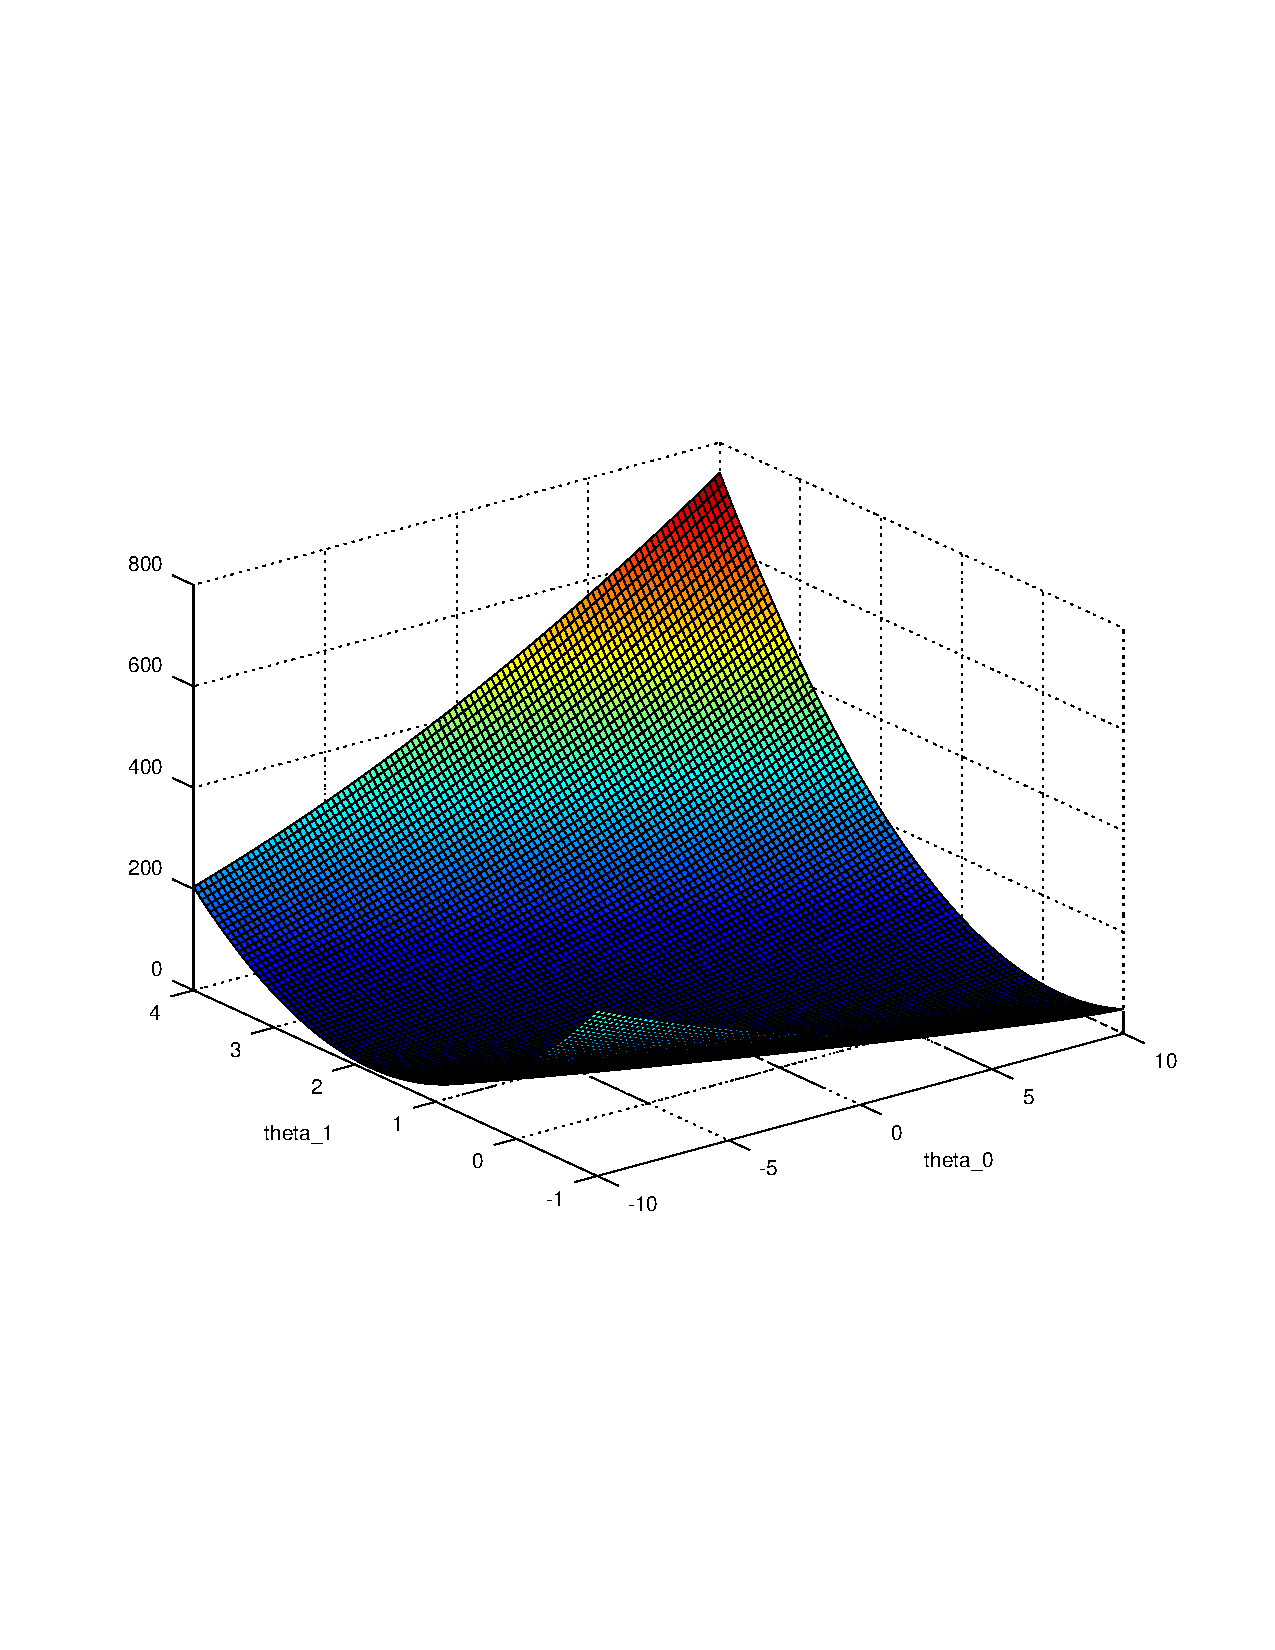
\includegraphics[width=\textwidth]{img/funcaodecustosurf}
    \caption{Gráfico de superfície}
  \end{subfigure} 
  %
  \begin{subfigure}[htb \label{fig:funcaodecustocontorno}]{0.5\textwidth}
    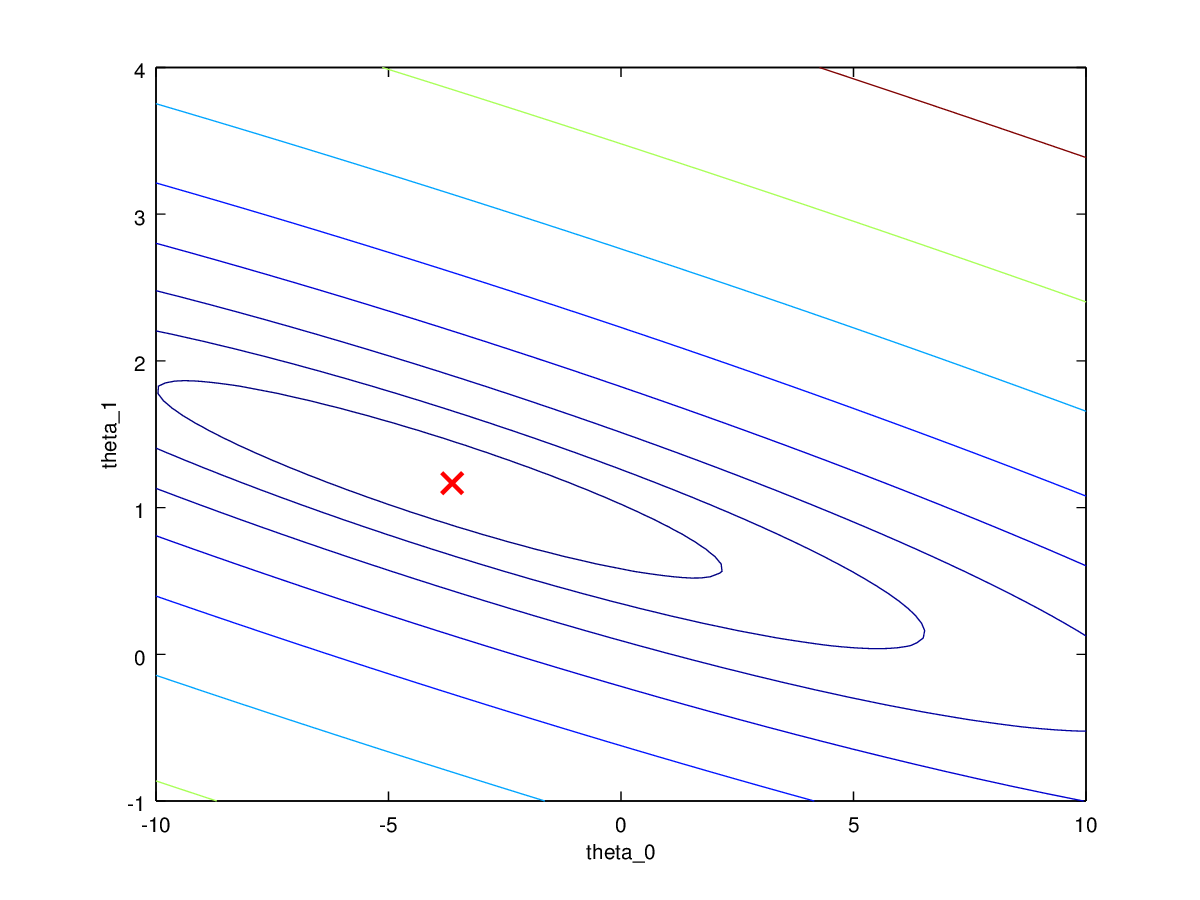
\includegraphics[width=\textwidth]{img/funcaodecustocontorno}
    \caption{Gráfico de contorno}
  \end{subfigure}
\end{figure}


\subsection{Minimização da função de custo}

Para essa tarefa é necessário a aplicação de um algoritmo que pega a função de custo e tente minimizá-la, e por fim retorne os valores dos parâmetros $ \theta $s aprendidos. Com isso, estaremos melhorando nossa função de hipótese. 

Um dos algoritmos mais utilizados para essa tarefa é o \textbf{Gradiente Descendente} [X], seu funcionamento baseia-se em seguir a derivida da função de custo em relação aos parâmetros $\theta$s alternadamente, com isso a encosta da tangente dará a direção para seguir adiante. Além disso, é aplicada uma taxa de aprendizagem $ \alpha $ a cada iteração, para tentar controlar a convergência.

Seu funcionamento é descrito pelo algoritmo \ref{eq:gradientedesc}.

\textit{repita até convergir \{}
\begin{equation}
\label{eq:gradientedesc}
\quad \theta_j := \theta_j = \alpha \frac{\partial}{\partial\theta_j} J(\theta)
\end{equation}
\textit{\quad\quad\quad \}}

Ao trabalhar sobre a derivada parcial da função de custo, podemos chegar na \autoref{eq:gradientefinal} e adiante na versão vetorizada na \autoref{eq:gradientefinalvet}. A explicação de como trabalhar sobre a derivada pode ser encontrado no \autoref{app:derivadagradiente}.

\begin{equation}
\quad \theta_j := \theta_j = \alpha \sum\limits_{i=1}^{m}\Big(h_{\theta}(x^{(i)}) - y^{(i)} \Big) x_j^{(i)} \label{eq:gradientefinal}
\end{equation}

\begin{equation}
\quad \theta := \theta - \frac{\alpha}{m}X^T(g(X\theta) - Y) \label{eq:gradientefinalvet}
\end{equation}

Na \autoref{fig:funcgraddesc} é possível visualizar esse funcionamento sobre os parâmetros. Observe que nesse caso o algoritmo consegue convergir para o mínimo global, porém em alguns casos (dependendo de nossa taxa de aprendizagem $ \alpha $) pode-se convergir para um mínimo local como mostrado na \autoref{fig:funcgraddescnot}

\begin{figure}
  \caption{Funcionamento do Gradiente Descendente}
  \begin{subfigure}[htb]{0.5\textwidth}
    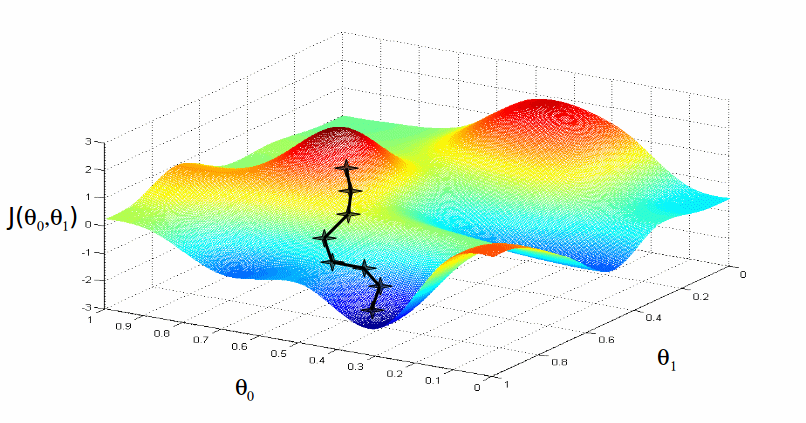
\includegraphics[width=\textwidth]{img/funcgraddesc1}
    \caption{Convergindo para uma mínimo global} \label{fig:funcgraddesc}
  \end{subfigure}
  %
  \begin{subfigure}[htb]{0.5\textwidth}
    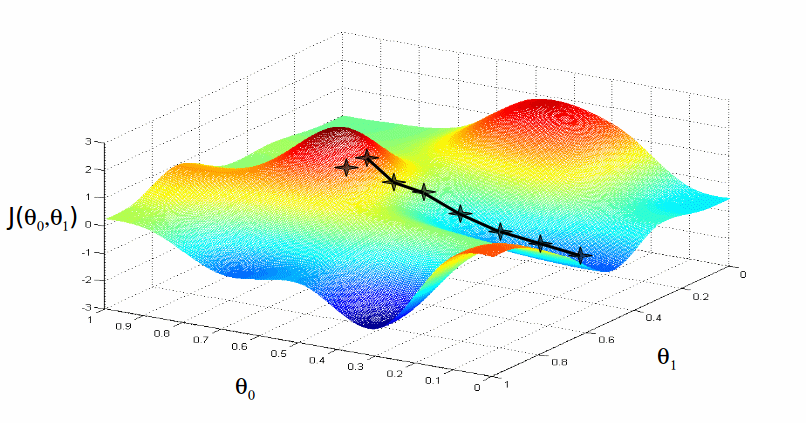
\includegraphics[width=\textwidth]{img/funcgraddesc2}
    \caption{Convergindo para uma mínimo local} \label{fig:funcgraddescnot}
  \end{subfigure}
\end{figure}

O Gradiente Descendente é apenas um dos vários algoritmos que existem para minimizar a função de custo. De acordo com [X] há alternativas mais sofisticadas como o Gradiente Conjugado, BFGS e L-BFGS, mas também é sugerido que não devemos tentar codificar esses algoritmos, visto que são difíceis e requerem um bom conhecimento de cálculo numérico.


\subsection{Classificação multiclasse}

O \ac{pos} Tagging é um problema de classificação multiclasse, onde deve-se etiquetar uma palavra em uma de várias categorias gramaticais possíveis. É possível fazer isso ao expandir nossa definição para que a saída seja $y = \{0, 1, ..., n\}$. Nesse caso, é dividido o problema em \textit{n + 1} problemas de classificação binária e em cada um será feito a predizagem da probabilidade de que $y$ é membro de uma dessas classes.
\begin{align}
h_{\theta}^{(0)}(X) =&  P(y=0 | X ; \theta) \nonumber \\
h_{\theta}^{(1)}(X) =&  P(y=1 | X ; \theta) \nonumber \\
\vdots & \nonumber \\
h_{\theta}^{(n)}(X) =&  P(y=n | X ; \theta) \nonumber
\end{align}

E então escolhe-se a classe com o valor de hipótese mais alto.
\begin{equation}
prediction = max_i(h_{\theta}^{(i)}(X)) \nonumber
\end{equation}


\subsection{Regularização}

Regularização é um conceito importante designado para resolver o problema de \textit{overfitting}.

Lorem ipsum dolor sit amet, consectetur adipisicing elit, sed do eiusmod
tempor incididunt ut labore et dolore magna aliqua. Ut enim ad minim veniam,
quis nostrud exercitation ullamco laboris nisi ut aliquip ex ea commodo
consequat. Duis aute irure dolor in reprehenderit in voluptate velit esse
cillum dolore eu fugiat nulla pariatur. Excepteur sint occaecat cupidatat non
proident, sunt in culpa qui officia deserunt mollit anim id est laborum.



\section{Córpus e seu conjunto de classes gramaticais}

Córpus são uma coleção de textos colocados como um só, eles são os exemplos de entrada para nosso treinamento. A qualidade e o tamanho desses córpus são importantes para que o etiquetador possa generalizar sentenças ainda não vistas. Eles contém também um conjunto de classes gramaticais associadas a cada palavra.

Esses conjuntos podem se diferenciar na sua granularidade, como por exemplo, podem ter diferentes classes gramaticais para nomes no plural e no singular, ou agrupar eles em uma única classe [X]. No inglês, há vários córpus de qualidade que são amplamento utilizados, são o Penn Treebank tagset [X], CLAWS5 [X] e CLAWS7 [X].

Já no português esses córpus estão evoluindo com o tempo, embora muitos erros são encontrados neles [X], eles ainda são a melhor opção devido a seu tamanho e qualidade, os principais e mais utilizados para essa tarefa são o Mac-Morpho [X] com cerca de um milhão de palavras, que retrata artigos publicados na Folha de São Paulo em 1994. O Tycho Brahe [X] que também tem cerca de um milhão de palavras e retrata assuntos históricos de 66 textos diferentes, a linguagem utilizada nele é muito diferente da usada no cotidiano e por isso o seu uso é apenas a fim de curiosidade. Temos também o Bosque [X], que contém cerca de 185 mil palavras. Além desses, [X] et al. apresenta uma versão revisada do Mac-Morpho, com classes gramaticais novas e junção de outras. 

Infelizmente esses córpus não podem ser combinados em um só, já que eles se diferenciam no conjunto de classes gramaticais e também no seu uso associado.

A aprendizagem baseada em córpus tem se mostrado uma estratégia atrativa, já que pode ser usado recursos criados com melhores performance [X, Y, Z]. Devido a isso, nesse trabalho vamos utilizar três córpus: o Mac-Morpho original; Mac-Morpho revisado e o Tycho Brahe. O conjunto de etiquetas para esses córpus podem ser encontrados, respectivamente, em [X], [Y] e [Z].


\textit{- Falar mais alguma coisa sobre?}

\textit{- Colocar alguma tabela aqui?}



\section{Representação das palavras}\label{sec:representacaodaspalavras}

Palavras \footnote{Uma palavra pode ser qualquer conjunto de caracteres, inclusive pontuações, números, etc.} podem ser representadas de várias maneiras em um modelo de aprendizagem, podendo ser até mesmo feito o uso real da palavra como um conjunto de caracteres.

No entanto, a melhor abordagem e a mais indicada atualmente é a utilização de \textit{word embeddings}, elas são representação de palavras como vetores reais valorados em um espaço multidimensional [X]. Elas podem ser geradas de maneiras diferentes dependendo da técnica utilizada, clássicas abordagens baseiam-se na frequência e co-ocorrência [X] das palavras, até mesmo via modelos de redes neurais [X]. Um dos processos de criação é mostrado na \autoref{fig:criacaowordemb}.

\begin{figure}[htb]
  \caption{Exemplo de criação de \textit{word embeddings}} \label{fig:criacaowordemb}
  \begin{center}
      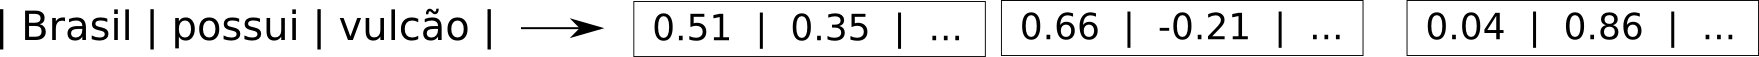
\includegraphics[scale=0.3]{img/criacaowordemb}
  \end{center}
\end{figure}


Ou seja, dada uma palavra \textit{word}, temos a transformação \textit{W}:
\begin{equation}
W:word \to \mathbb{R}^n
\end{equation}

Em ordem de prever esses valores com precisão, a rede precisa aprender bons parâmetros para \textit{W}.

A grande vantagem em se utilizar \textit{word embeddings} é o fato dessa técnica conseguir capturar informações sintáticas e semânticas das palavras. Isso pode ser visualizado através do t-SNE [X], uma técnica sofisticada para visualizar dados em altas dimensões.

\begin{figure}[htb]
  \caption{t-SNE: Visualização para \textit{word embeddings}}\label{fig:wordtsne}
  \begin{center}
      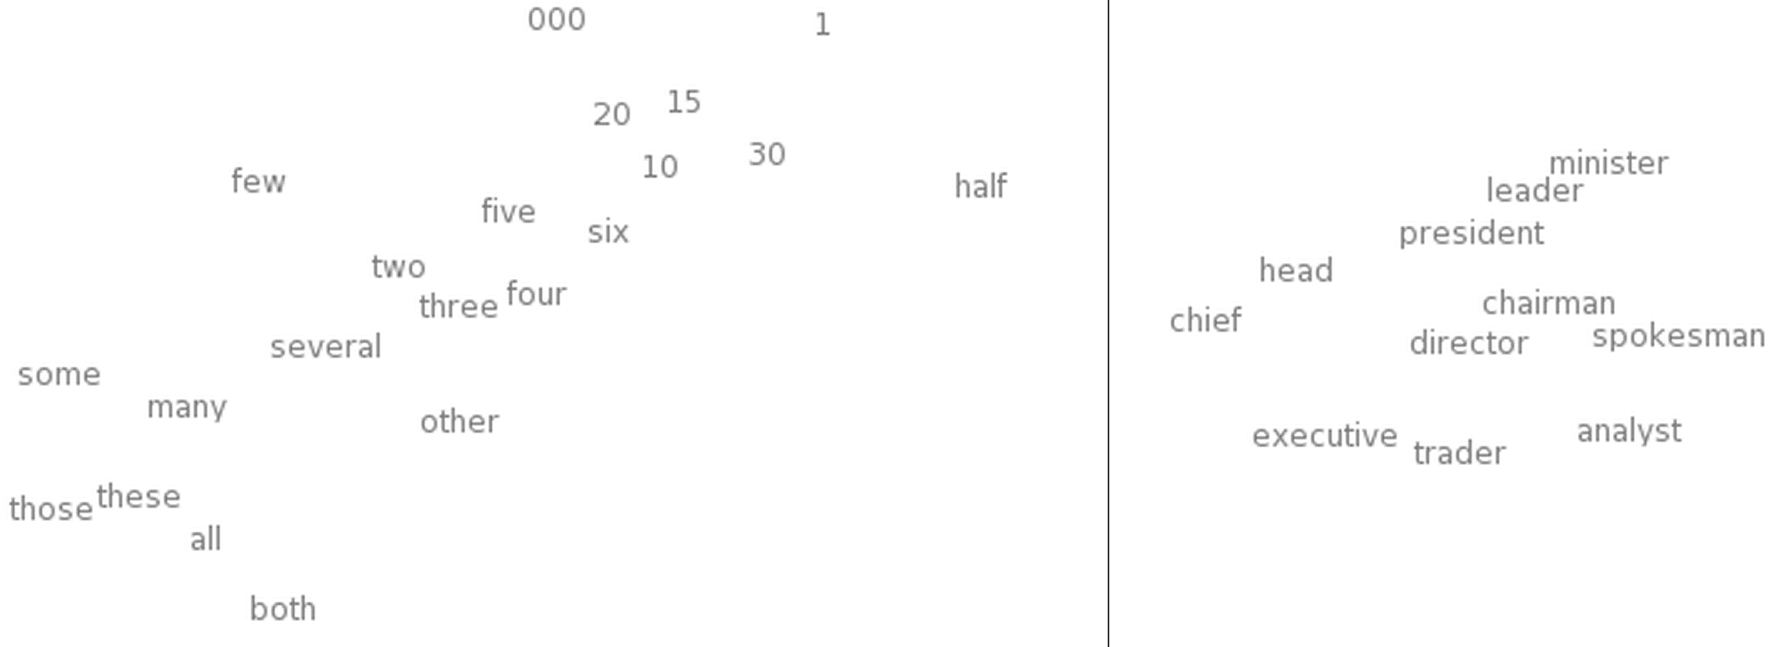
\includegraphics[scale=0.25]{img/Turian-WordTSNE}
  \end{center}
  \legend{Fonte: Turian et al. (2010).}
\end{figure}

Na \autoref{fig:wordtsne} podemos visualizar um tipo de mapeamento entre os sentidos intuitivos das palavras, onde na esquerda estão palavras referentes a números e na direita palavras referentes a profissões. Ou seja, palavras similares estão pertos umas das outras.

\begin{figure}[htb]
  \caption{Exemplo de palavras similares}\label{fig:palavrassimilares}
  \begin{center}
      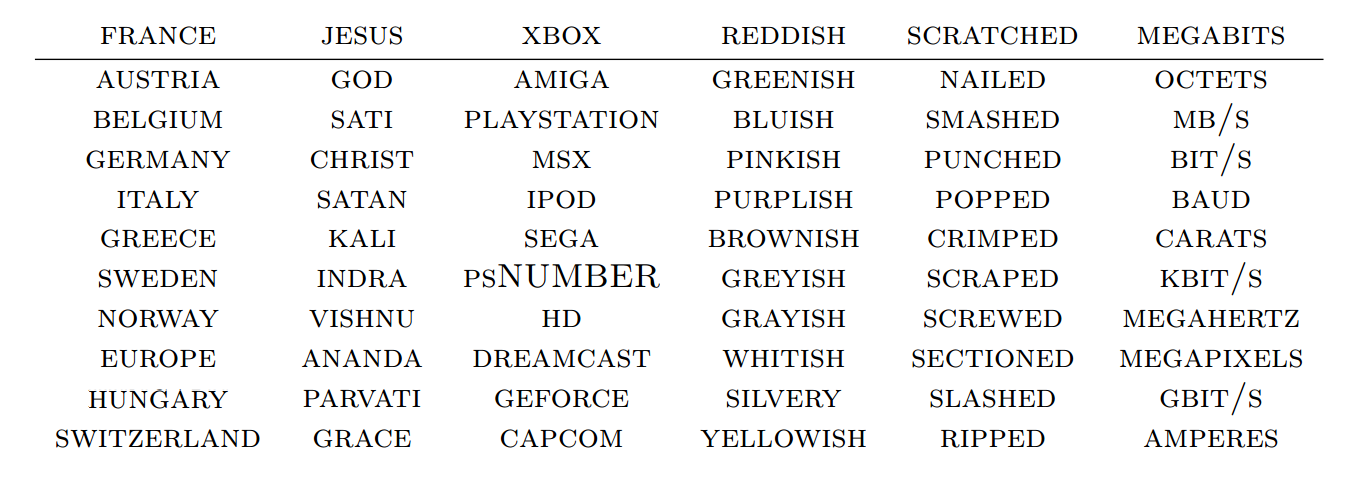
\includegraphics[scale=0.25]{img/Colbert-WordTable2}
  \end{center}
  \legend{Fonte: Collobert et al. (2011)}
\end{figure}

Na \autoref{fig:palavrassimilares} temos mais alguns exemplos desse conceito, com isso podemos realizar tarefas semânticas mais facilmente, como o exemplo \ref{eq:exemploobjetivo}, que é o que esperamos obter.

Para mais informações sobre \textit{word embeddings} consultar [X] e [Y].



\section{Redes neurais profundas}

O que escrever aqui? 

- Conceitos basicos de redes neurais

- Redes neurais profundas e seus algoritmos

